\section{A research agenda in AI for
science}\label{a-research-agenda-in-ai-for-science}

`AI for science' sits at a nexus of disciplines, methods, and
communities. Both AI and `science' (broadly defined) share a core
interest in learning from data. From this interest emerge different
research directions: for AI, questions about the nature of intelligence
and how to understand the learning process in humans and machines; for
science, the outputs of this learning process are the focus, with the
aim of adding new knowledge about natural, physical, and social systems.
A distinctive feature of the emerging `AI for science' agenda is the
ability to move between these worlds, using AI to drive progress in
science and taking inspiration from science to inspire progress in AI.
The result is a continuum of modelling approaches along a spectrum from
strongly mechanistic to statistical models, which allow researchers to
introduce or operate at different levels of abstraction.

The AI for science community therefore combines the ambitions of AI
research with domain-specific goals to advance the frontiers of research
and innovation in their discipline, with an engineering focus on
designing systems that work in deployment, while operating across scales
from the nano- to the interstellar. From these interfaces emerges a
research agenda that -- if successful -- promises to accelerate progress
across disciplines. Inspired by discussions at the Dagstuhl workshop, a
list of research questions arising from this agenda is given in Annex 2.
These span three themes:

\emph{\textbf{Building AI systems for science:}} Attempts to deploy AI
in the context of scientific discovery have exposed a collection of gaps
in current machine learning and AI capabilities. Further work is needed
to develop the technical capabilities that will allow AI to be used more
effectively in research and innovation; developing those capabilities
also offers opportunities to contribute to wider attempts to deliver
sophisticated AI systems. Areas for progress include:

\begin{itemize}
\item
  Advancing methods, software and toolkits for high-quality simulation
  and emulation, which integrate effective uncertainty quantification
  and leverage advances in machine learning robustness to ensure the
  operate safely and effectively.
\item
  Detecting scientifically meaningful structure in data, through
  advances in causal machine learning.
\item
  Encoding domain knowledge in AI systems through integration of
  scientific laws, principles, symmetries, or invariances in machine
  learning models, and through virtual, autonomous systems to make
  research more effective.
\end{itemize}

\emph{\textbf{Combining human and machine intelligence:}} Effective
deployment of AI in science requires effective interactions between
human, domain and machine intelligence across all stages of the
deployment pathway. AI systems can be made more effective by integrating
pre-existing knowledge about the system of study, but mechanisms are
needed to extract and encode that knowledge. Effective interfaces are
also required in the reverse direction. Translating the outputs of AI
analysis to increased human capability requires an understanding of what
insights are relevant, how they are best communicated, and the cultural
environment that shapes the conduct of science. Areas for progress
include:

\begin{itemize}
\item
  Designing interfaces between humans and machines or AI agents that can
  extract, formalise, and assimilate knowledge that domain researchers
  have acquired, including tacit knowledge, and that communicate new
  knowledge back to the user as actionable insights.
\item
  Building mechanisms for explainability that allow researchers to
  interrogate why and how an AI system delivered a particular result,
  with the explanations provided being tailored to user need.
\item
  Accelerating the pace of knowledge creation and use, through systems
  that mine the existing research knowledge base or that automate
  repetitive or time-consuming elements of the research process.
\end{itemize}

\emph{\textbf{Influencing practice and adoption:}} By learning from
recent experiences of deploying AI for science, the field has an
opportunity to promote wider uptake and progress in both scientific
domains and in AI research. This requires capturing both the knowledge
that the community has already generated, about how to design AI
systems, and the know-how about how to overcome practical challenges
that accompanies it, while taking action to grow the community of
researchers excited about the potential of AI in science. Areas for
progress include:

\begin{itemize}
\item
  Supporting new applications, through challenge-led research programmes
  that promote interdisciplinary collaborations and support co-design of
  AI systems to help tackle scientific challenges.
\item
  Developing toolkits and user guides that allow researchers to
  understand which AI tools are suitable for which purposes, and how to
  deploy those tools in practice.
\item
  Sharing skills and know-how, through community outreach that
  disseminates knowledge and know-how in how to use AI.
\end{itemize}

Together, these areas for action highlight the importance of interfaces
-- between researchers and between modelling approaches -- in shaping
the development of AI for science (Figure 3).

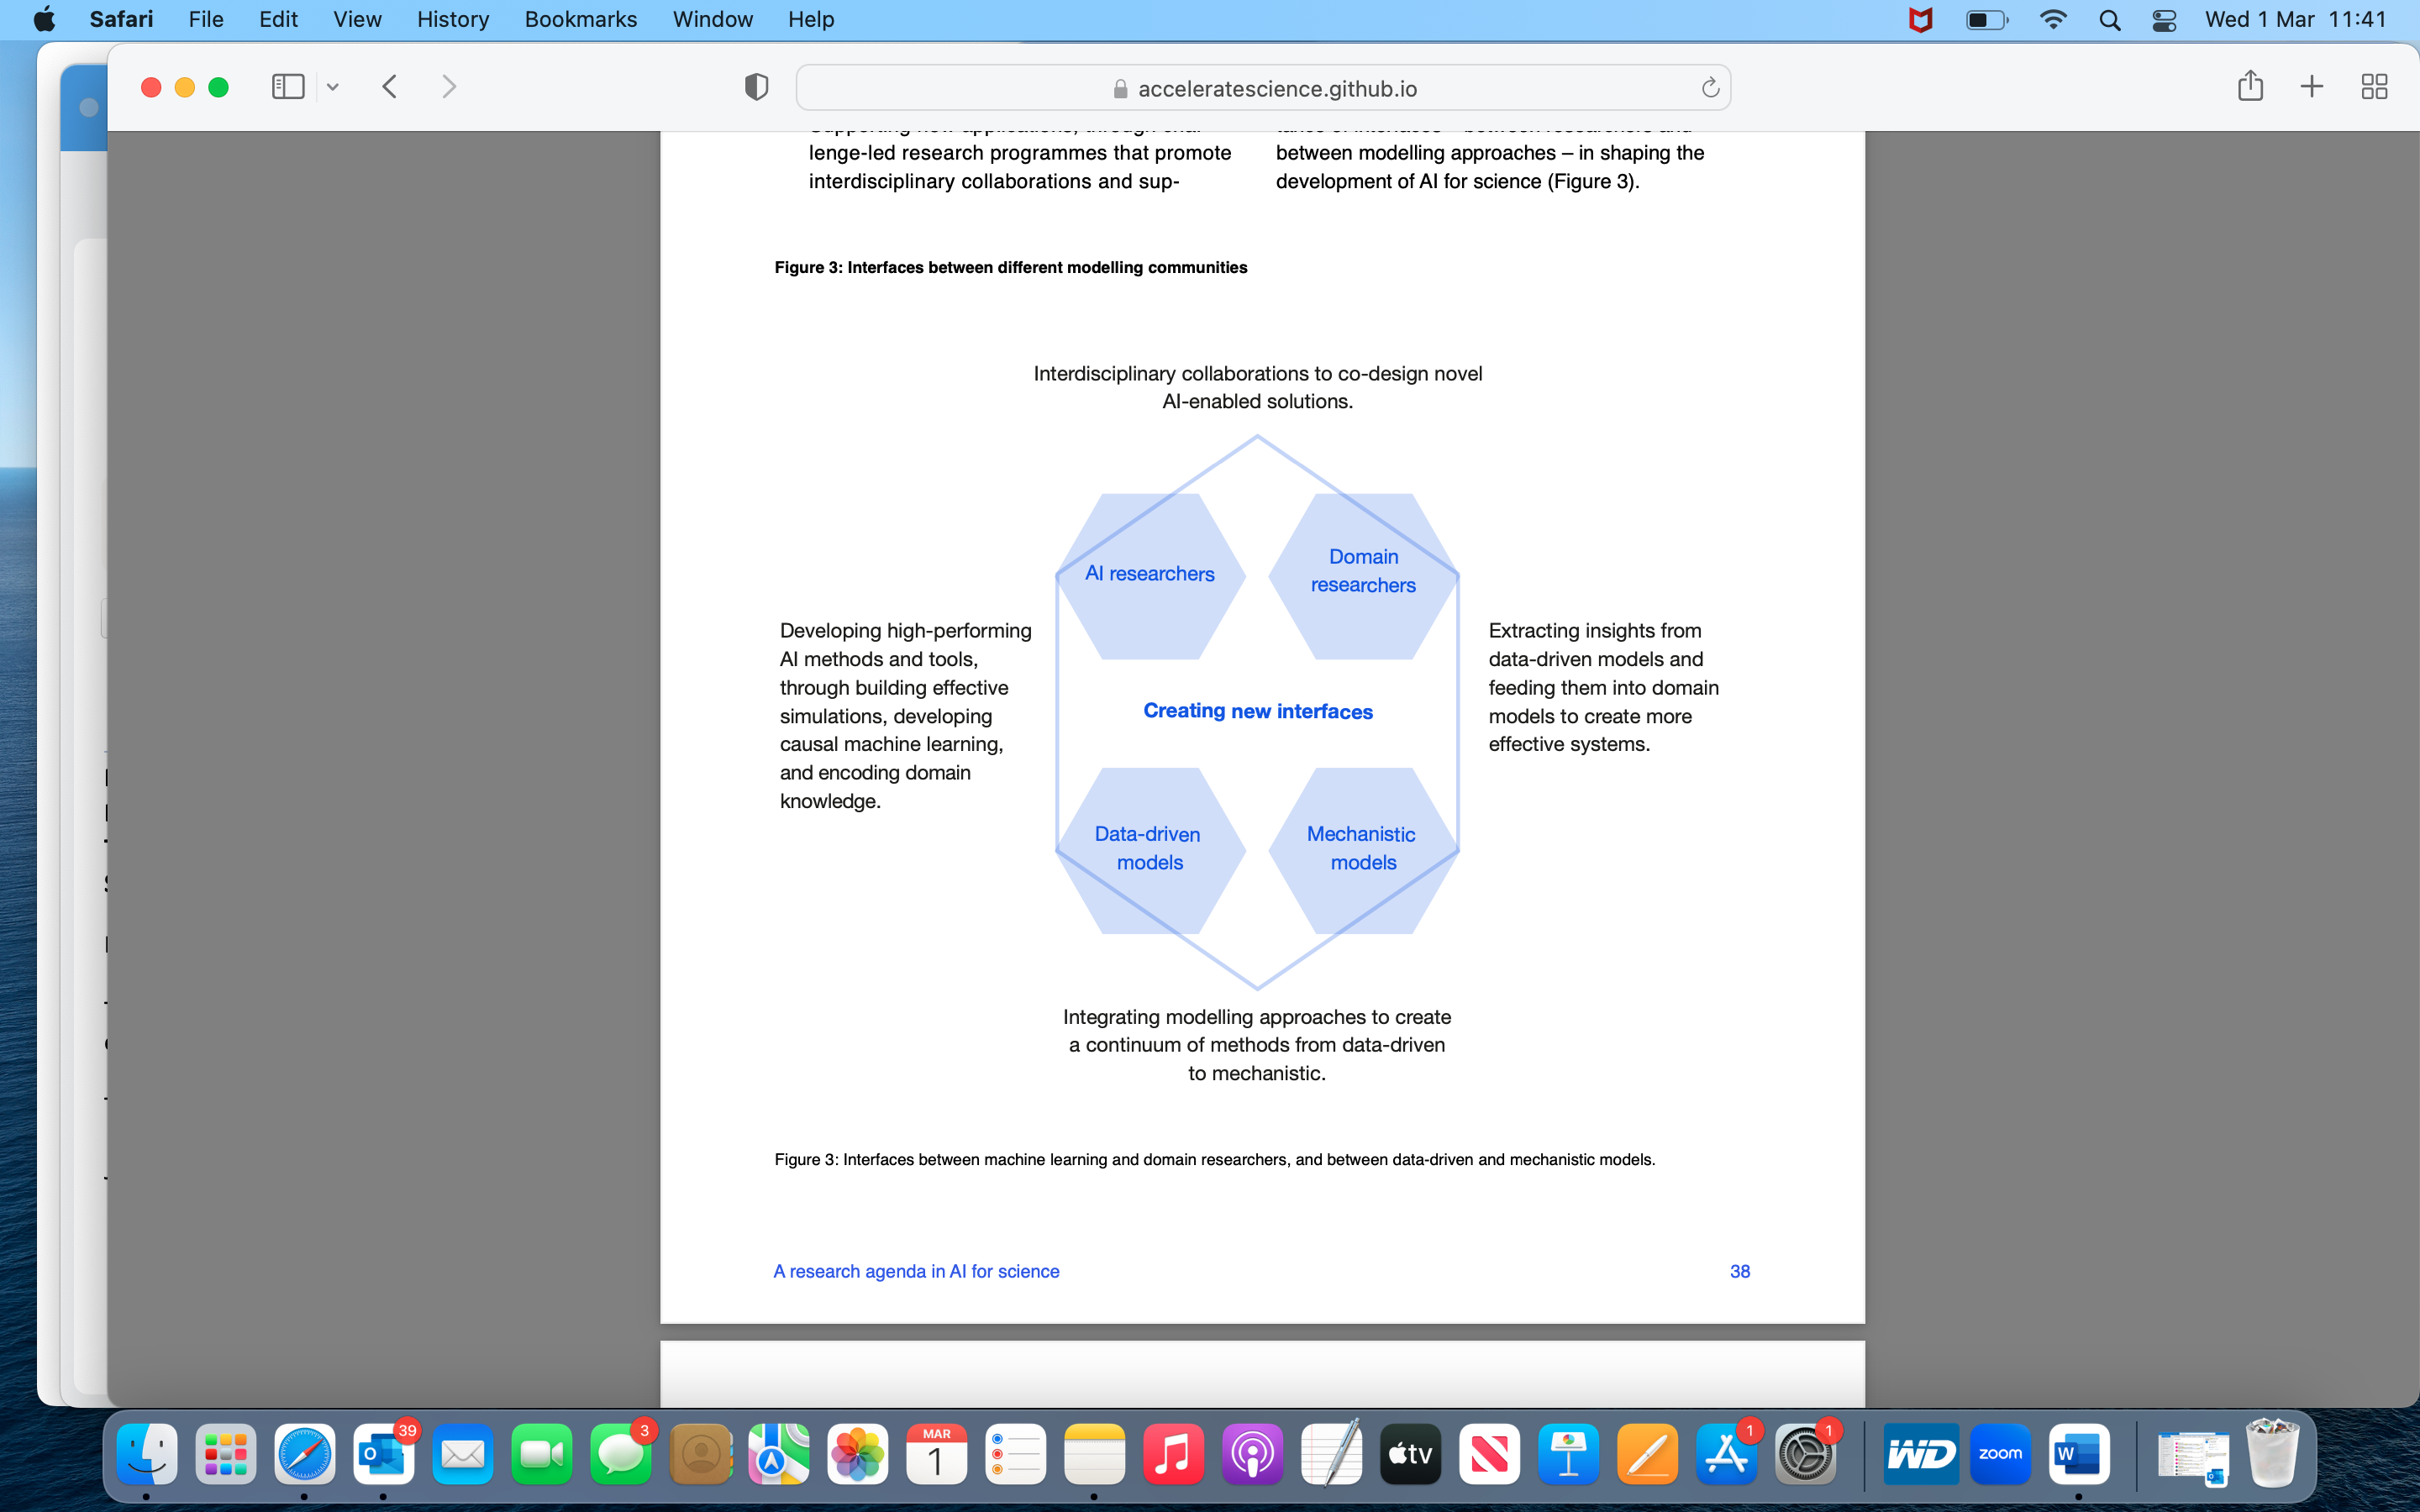
\includegraphics[width=5.98951in,height=5.6132in]{media/image3.png}

\hypertarget{accelerating-progress-in-ai-for-science}{%
\section{\texorpdfstring{Accelerating progress in AI for science
}{Accelerating progress in AI for science }}\label{accelerating-progress-in-ai-for-science}}

Building on the impressive advances that machine learning has already
supported in many domains, widespread adoption of AI for research has
the potential to catalyse a new wave of innovations that in turn could
drive greater health, wealth, and wellbeing. The question facing
researchers, funders, and policymakers today is how to harness that
potential. The challenge is to build capability across the research
landscape, connect areas of expertise to areas of need, and to
accelerate the transfer of successful ideas between domains.

The experiences of deploying AI for science described in this document,
and the research agenda that results from these experiences, suggest a
roadmap for action. That roadmap charts a pathway to create an enabling
environment for AI in science, by advancing research that delivers AI
methods to support scientific discovery, building tools and resources to
make AI accessible, championing interdisciplinary research and the
people pursuing it, and nurturing a community at the interface of these
different domains. Progress across these areas can unlock scientific and
methodological advances in AI for science, while also helping answer an
emerging question about whether there exists a core discipline of `AI
for science'. The shared themes and interests that emerge from research
projects at the interface of AI and scientific domains suggest that
there is potential for `AI for science' to surface as a distinct
speciality in computer science. In parallel, domain-specific efforts to
drive the adoption of AI as an enabler of innovation are also needed to
deliver the benefits of AI for scientific discovery.

\hypertarget{advance-new-methods-and-applications}{%
\subsection{Advance new methods and
applications}\label{advance-new-methods-and-applications}}

Efforts to deploy AI in the context of research have highlighted
cross-cutting challenges where further progress in AI methods and theory
is needed to create tools that can be used more reliably and effectively
in the scientific context. Effective simulations are needed to study the
dynamics of complex systems; causal methods to understand why those
dynamics emerge; and integration of domain knowledge to relate those
understandings to the wider world. While elements of these research
challenges are shared with other fields -- topics such as robustness,
explainability, and human-machine interaction also come to the fore in
fields such as AI ethics, for example -- they share an intersection in
the use of AI for science, in the context of efforts to bridge
mechanistic and data-driven modelling.

Alongside these `AI' challenges are a collection of `science'
challenges, where researchers, policymakers and publics have aspirations
for AI to deliver real-world benefits.\footnote{See, for example: the
  EU's Innovation Missions
  \href{https://research-and-innovation.ec.europa.eu/funding/funding-opportunities/funding-programmes-and-open-calls/horizon-europe/eu-missions-horizon-europe_en}{\uline{https://research-and-innovation.ec.europa.eu/funding/funding-opportunities/funding-programmes-and-open-calls/horizon-europe/eu-missions-horizon-europe\_en}}
  and UN SDG's
  \href{https://sdgs.un.org/goals}{\uline{https://sdgs.un.org/goals}}}
Such challenges offer the opportunity to accelerate progress in AI,
while facilitating interdisciplinary exchanges, and opening the field to
input from citizen science or other public engagement initiatives. In
developing these research missions, care is needed to define
cross-cutting questions or challenges that broaden scientific
imaginations, rather than restricting them. The process of converting a
complicated scientific problem into something tractable with AI
necessarily involves some narrowing of focus; to be successful,
mission-led innovation efforts must achieve this focus without losing
meaning, or creating benchmarks that misrepresent the complexity of the
real-world challenge.

Defining shared challenges could help rally the AI for science community
and drive progress in both methods and applications of AI in science.
There already exists examples of how such challenges can build
coalitions of researchers across domains from which the field can draw
inspiration. These include the GREAT08 project, which developed image
analysis techniques to study gravitational lensing;\footnote{Bridle, S.,
  Balan, S.T., Bethge, M., Gentile, M., Harmeling, S., Heymans, C.,
  Hirsch, M., Hosseini, R., Jarvis, M., Kirk, D., Kitching, T., Kuijken,
  K., Lewis, A., Paulin-Henriksson, S., Schölkopf, B., Velander, M.,
  Voigt, L., Witherick, D., Amara, A., Bernstein, G., Courbin, F., Gill,
  M., Heavens, A., Mandelbaum, R., Massey, R., Moghaddam, B., Rassat,
  A., Réfrégier, A., Rhodes, J., Schrabback, T., Shawe-Taylor, J.,
  Shmakova, M., van Waerbeke, L., Wittman, D. (2010) Results of the
  GREAT08 Challenge: an image analysis competition for cosmological
  lensing, \emph{Monthly Notices of the Royal Astronomical Society},
  Volume 405, Issue 3, July 2010, Pages 2044--2061,
  \href{https://doi.org/10.1111/j.1365-2966.2010.16598.x}{\uline{https://doi.org/10.1111/j.1365-2966.2010.16598.x}}}
the Open Problems in Single Cell Biology challenge, which convened the
machine learning community to make progress in Multimodal Single-Cell
Data Integration;\footnote{For further information, see:
  https://openproblems.bio/neurips\_2021/} and the SENSORIUM challenge,
focused on advancing understandings of how the brain processes visual
inputs.\footnote{For further information, see:
  https://sensorium2022.net/home} In pursuing this agenda, researchers
can leverage well-established protocols in open-sourcing materials and
sharing documentation to help ensure research advances are rapidly and
effectively disseminated across disciplines. The result should be more
effective methods, and an agile research environment where researchers
can flex methods across disciplines.

\hypertarget{invest-in-tools-and-toolkits}{%
\subsection{Invest in tools and
toolkits}\label{invest-in-tools-and-toolkits}}

Complementing these efforts to build and share knowledge, well-designed
software tools can help make accessible the craft skills (or know-how)
that make AI for science projects successful. Modelling is a core
component of all AI for science projects. In some aspects, the task for
the field can be thought of as charting a path between the statistician,
whose effectiveness comes from proximity to the domain but whose methods
struggle to scale, and the mathematician, whose tools are adopted across
domains but with some loss of meaning as the distance between
method-generator and adopter increases.

The energy already invested in building effective machine learning
models can be leveraged for wider progress across domains through
investment in toolkits that support the generalisation of effective
approaches. Wide-spectrum modelling tools could offer `off the shelf'
solutions to common AI for science research questions. The challenge for
such toolkits is to create an effective interface between tool and user.
Connecting with the field of human-computer interaction could generate
design insights or protocols to help create more effective human-AI
interfaces.

Best practices in software engineering can help, through documentation
that supports users to successfully deploy modelling tools. User guides
-- or taxonomies of which models are best suited for which purposes and
under what circumstances -- can also help make accessible to non-expect
users the accumulated know-how that machine learning researchers have
gained through years of model development and deployment.

A related engineering challenge is that of data management and
pipeline-building. To interrogate how a model works, why a result was
achieved, or whether an AI system is working effectively, researchers
often benefit from being able to track which data contributed to which
output. The data management best practices that allow such tracking need
to be embedded across AI for science projects. Data management
frameworks -- such as the FAIR data principles -- have already been
developed with the intention of making data more available, and useful,
for research. Further investment is now needed in efforts to implement
those principles in practice.

Investment in these foundational tools and resources can help build
understanding of which AI methods can be used and for what purposes,
lowering the barriers to adopting AI methods across disciplines.

\hypertarget{build-capability-across-disciplines}{%
\subsection{Build capability across
disciplines}\label{build-capability-across-disciplines}}

Central to progress in both research and toolkit engineering is the
availability of talented researchers with a passion for advancing
science through AI. People matter at all stages of the AI development
and deployment pipeline. Successful projects rely on researchers who are
motivated to work at the interface of different domains; collaborators
who can explain and communicate core concepts in their work across
disciplinary boundaries; engineers who can translate the needs of
different users into AI toolkits; and convenors that can inspire wider
engagement with the AI for science agenda.

Building these capabilities requires multiple points of engagement.
Domain researchers need access to learning and development activities
that allow them to understand and use foundational methods in machine
learning, whether as formal training or through the availability of
tutorials or user guides. AI researchers need access to the scientific
knowledge that should shape the methods they develop, the skills to
translate their advanced knowledge to materials that can be shared for
wider use, and the capacity to dedicate time and resource to learning
about domain needs.\footnote{A comparison here can be drawn with the
  development of statistics as an enabling discipline for many domains:
  statisticians have devoted time to understanding domain practices and
  integrating their work within those practices, often dedicating
  significant resource to understand the nature of the datasets with
  which they are working, before introducing modelling ideas.} Both need
skills in communication, organisation, and convening to operate across
disciplines. Without such capability-building, disciplines risk
remaining siloed; domains developing unrealistic expectations about what
AI can deliver in practice, and AI losing touch with the scientific
questions that are most meaningful to domains.

Institutional incentives shape how individuals engage (or not) with such
interdisciplinary exchanges. Interdisciplinary research often takes
longer and lacks the outlets for recognition available to those working
in single domains, affecting both the motivation of and opportunities
for career progression that are open to those working at the interface
of different disciplines. Much of the engineering work required to make
data and AI accessible beyond a specific project and useful to a wider
community is also traditionally unrecognised by academic incentive
structures. Aligning individual and institutional incentives in support
of interdisciplinarity is a long-standing challenge in research, and one
that becomes more critical to address in the context of developments in
AI. In this context, there may be new opportunities to recognise and
reward successes in AI for science, whether through new fellowships,
prizes, or ways of promoting the work done by those at this interface.

\hypertarget{grow-communities-of-research-and-practice}{%
\subsection{Grow communities of research and
practice}\label{grow-communities-of-research-and-practice}}

The areas for action described above feed into and from each other.
Progress in research and application can be leveraged to inspire a
generation of researchers to pursue interdisciplinary projects;
effective toolkits can make such progress more likely; skills-building
initiatives can prime researchers to be able to use these toolkits; and
so on, to create an environment where researchers and research advances
transition smoothly across disciplines, leading to a rising AI tide that
lifts all disciplines. Communities of research and practice are the
backdrop for creating such positive feedback loops.

A collection of AI for science initiatives are already building links
across the research landscape. The Machine Learning for Science Cluster
of Excellence at the University of Tübingen is leveraging the strength
of its local ecosystem in AI to drive wider progress in research and
innovation;\footnote{Programme website available at:
  \href{https://uni-tuebingen.de/en/research/core-research/cluster-of-excellence-machine-learning/home/}{\uline{https://uni-tuebingen.de/en/research/core-research/cluster-of-excellence-machine-learning/home/}}}
the Accelerate Programme for Scientific Discovery at the University of
Cambridge is building bridges across disciplines, building a community
passionate about opportunities in AI for science;\footnote{Programme
  website available at:
  \href{https://acceleratescience.github.io}{\uline{https://acceleratescience.github.io}}}
the University of Copenhagen's SCIENCE AI Centre provides a focal point
for AI research and education in its Faculty for Science;\footnote{Programme
  website available at:
  \href{https://ai.ku.dk}{\uline{https://ai.ku.dk}}} New York
University's Center for Data Science hosts interdisciplinary faculty
pursuing innovative research and education;\footnote{Programme website
  available at: \href{https://cds.nyu.edu}{\uline{https://cds.nyu.edu}}}
the University of Wisconsin-Madison's American Family Insurance Data
Science Institute is developing strategic partnerships to accelerate the
use of data science in research;\footnote{Programme website available
  at:
  \href{https://datascience.wisc.edu/institute/}{\uline{https://datascience.wisc.edu/institute/}}}
new investments by Schmidt Futures across a network of research
institutions are supporting new postdoctoral fellowships at the
interface of AI and sciences.\footnote{Schmidt Futures (2022) Schmidt
  Futures Launches \$148M Global Initiative to Accelerate AI Use in
  Postdoctoral Research, available at:
  \href{https://www.schmidtfutures.com/schmidt-futures-launches-148m-global-initiative-to-accelerate-ai-use-in-postdoctoral-research/}{\uline{https://www.schmidtfutures.com/schmidt-futures-launches-148m-global-initiative-to-accelerate-ai-use-in-postdoctoral-research/}}}
Together, these initiatives demonstrate the appetite for progress in AI
for science.

There is an opportunity today to leverage these emerging interests into
a wider movement. Existing initiatives can drive capability-building, by
making training and user guides open, reaching out to engage domain
researchers in skills-building activities, and fostering best practice
in software and data engineering across disciplines. The links they
establish across research domains can form the basis of new
communication channels, whether through discussion forums, research
symposia, or newsletters to share developments at the interface of AI
and science. These communications can be deployed to raise the profile
of people and projects at this interface, celebrating successes, sharing
lessons, and demonstrating the value of interdisciplinary work.
Together, they can help develop an infrastructure for AI in science.

That infrastructure may also benefit from new institutional
interventions to address long-standing challenges in interdisciplinary
AI. New journals could provide an outlet to publish and recognise
high-quality AI for science research, bringing in contributions from
multiple disciplines and helping translate lessons across areas of work.
Membership organisations could help foster a sense of belonging and
community for researchers working at the interface of AI, science, and
engineering, developing career pathways and incentives. Efforts to
convene across disciplines can also catalyse new connections and
collaborations.

Emerging from these efforts is a paradigm shift in how to drive progress
in science. Historically, a small number of foundational texts have been
the catalyst that changed how researchers studied the world; Newton's
Principia; Darwin's Origin of Species; and so on. For much of its modern
history, scientific knowledge has been transmitted through textbooks;
canonical descriptions of the current state of knowledge. Today, the
transformative potential of AI is driven by its pervasiveness; its
impact in science will be achieved through integration across
disciplines. This integration requires widespread mobilisation,
convening machine learning researchers, domain experts, citizen
scientists, and affected communities to shape how AI technologies are
developed and create an amenable environment for their deployment. It
takes a community.

\hypertarget{ai-and-science-building-the-interface}{%
\subsection{AI and science: building the
interface}\label{ai-and-science-building-the-interface}}

Advances in AI have disrupted traditional ways of thinking about
modelling in science. Where researchers might previously have
conceptualised models as mechanistic -- reflecting known forces in the
world -- or data-driven, the `AI for science' methods that are emerging
today reject this separation. They are both, combining insights from
mechanistic and data-driven methods, integrating methods to create
something new. What follows from these developments is a spectrum of
modelling approaches, which researchers can deploy flexibly in response
to the research question of interest.

Today, the field of AI for science is characterised by intersections.
Between AI and scientific domains; between science and engineering;
between knowledge and know-how; between human and machine. It operates
across disciplinary boundaries, across scales from the atomic to the
universal, and across both the mission to understand intelligence and
the quest to deploy human intelligence to understand the world. Emerging
from these missions is a continuum of models and methods that allow
researchers to work across domains, extracting the knowledge that humans
have acquired, and levels of inquiry, enhancing that knowledge and
returning it in actional form.

As both a domain itself and an enabler of other disciplines, the power
of AI in science lies in its ability to convene diverse perspectives in
ways that accelerates progress across research areas. AI for science is
a rendezvous point. Its next wave of development will come from taking
strength from its diversity, and bringing more people into its
community.
